%%%%%%%%%%%%%%%%%%%%%%%%%%%%%%%%%%%%%%%%%%%%%%%%%
%
%  problems remaining:
%  #  why the z-vector equation only solved once? we do not need to solve 3N
%      equations?
%
%
%
%
%
%



\chapter{Configuration Interaction Singles Method}
%
%
%
%
In the configuration interaction method, the most easiest way is to just take
the first excitation states into consideration. Such method is called
``Configuration Interaction Singles Method'', so it's abbreviated as
``CIS'' method.

%%%%%%%%%%%%%%%%%%%%%%%%%%%%%%%%%%%%%%%%%%%%%%%%%
\section{CIS Formulation}
%
%
%
%
Firstly, let's go to investigate the formulation to calculate the CIS
energy. In the first step, we will only consider the restricted type
of determinants so that to make things easier. 

Suggest we have $n$ occupied MOs, and the electrons are $2n$; then the
ground state Slater determinant is:
\begin{equation}
  \label{eq:CISeq:1}
  \Phi_{HF} =  |\varphi_{1}(1)\alpha(1)\varphi_{1}(2)\beta(2)\cdots
\varphi_{n-1}(2n-1)\alpha(2n-1)\varphi_{n}(2n)\beta(2n)|  
\end{equation}

It's energy is:
\begin{multline}\label{CISeq:2}
% \nonumber to remove numbering (before each equation)
  E
  =\sum_{i}^{occ}\langle\varphi_{i}(1)|\hat{h}_{1}|\varphi_{i}(1)\rangle
  +  \\
  \sum_{i < j}^{occ} \left\{
    2\langle\varphi_{i}(1)\varphi_{j}(2)|\frac{1}{r_{12}}|\varphi_{i}(1)\varphi_{j}(2)\rangle-
    \langle\varphi_{i}(1)\varphi_{j}(2)|\frac{1}{r_{12}}|\varphi_{j}(1)\varphi_{i}(2)\rangle
  \right\}
\end{multline}

More specifically, the energy for the orbital is (here we suppose that
the orbital is in $\alpha$ spin state):
\begin{eqnarray}\label{CISeq:3}
% \nonumber to remove numbering (before each equation)
  \epsilon_{i} &=&  \langle \varphi_{i}| \hat{F} | \varphi_{i} \rangle \nonumber \\
  &=& \langle i|h|i \rangle + \sum_{j \neq i} \left\{
    2[ii|jj] - [ij|ij]
  \right\}
\end{eqnarray}
This is for the occupied orbital, so we have to specify that $j \neq
i$. For the virtual orbital, it's energy is:
\begin{eqnarray}\label{CISeq:4}
% \nonumber to remove numbering (before each equation)
  \epsilon_{a} &=&  \langle \varphi_{a}| \hat{F} | \varphi_{a} \rangle \nonumber \\
  &=& \langle a|h|a \rangle + \sum_{j}^{occ} \left\{
    2[aa|jj] - [aj|aj]
  \right\}
\end{eqnarray}
Here we note that we use a, b, c etc. to designate the virtual
orbitals, the i, j, k etc. to refer to the occupied orbitals; and p,
q, r etc. to specify the general orbitals.

Now through the HF calculation, we have gotten $n$ occupied orbitals
and another $m$ virtual orbitals ($n+m$ is the number of basis
sets). The next question is, how to form the single excitation states
from HF orbitals?

In this process, an electron from the occupied orbital is ``fired up''
into some virtual orbitals, so that to form some new determinant. Then
the new Slater determinant can be expressed as:
\begin{equation}
    \label{eq:CISeq:5}
  \Phi_{i}^{a} =  |\cdots\varphi_{a}(k)\alpha(k)\varphi_{i}(k+1)\beta(k+1)\cdots
\varphi_{n-1}(2n-1)\alpha(2n-1)\varphi_{n}(2n)\beta(2n)|  
\end{equation}
Here the electron $k$ with spin state of $\alpha$ is excited into the
virtual orbital $\varphi_{a}$, so we use the $\varphi_{a}$ to replace
the original $\varphi_{i}$ in the $\alpha$ spin state (see the picture
of \ref{ris_pic}). 
\begin{figure}[htbp]
\begin{center}
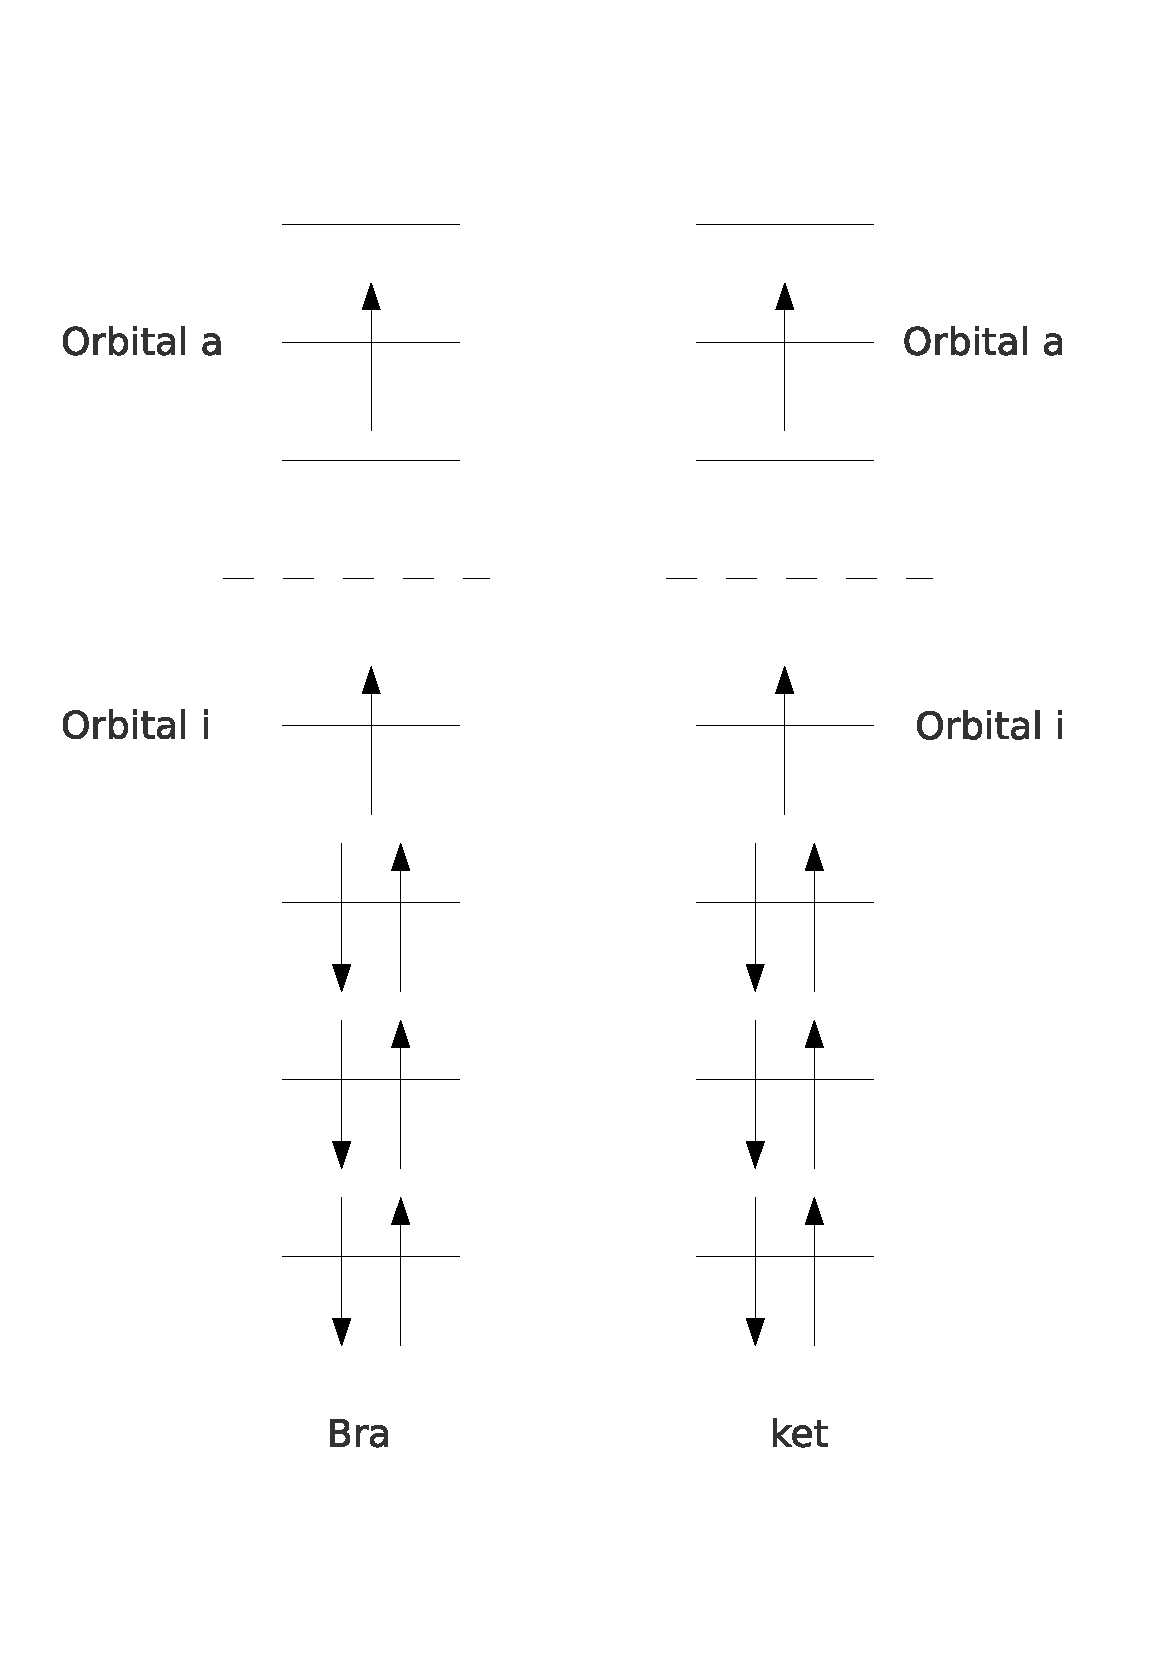
\includegraphics[scale=0.3]{ris1.eps}\label{ris_pic}
\caption{single excitation state}
\end{center}
\end{figure}

By such configuration method, actually we can form $n\times m$ Slater
determinants. Then the trial wave function can be expressed as their
linear combinations:
\begin{equation}
  \label{CISeq:6}
  \Psi = \sum_{i}^{occ}\sum_{a}^{vir}C_{i}^{a}\Phi_{i}^{a}
\end{equation}

Here there are two points should be clarified. Firstly, we note that
in the expression of (\ref{CISeq:6}) the root determinant (ground
state determinant) is not included. Why?

This reason for this is from Brillouin theorem, which has been
demonstrated in the above content. The Brillouin theorem says that the
HF determinant is unable to mix with the single excitation states, so
there's no coupling between them. If we include the HF determinant
into the expression of (\ref{CISeq:6}), the Hamiltonian matrix will be
just like the form below:
\begin{equation}
  \label{CISeq:7}
  \begin{bmatrix}
    \langle\Phi_{HF}|\hat{H}|\Phi_{HF}\rangle & 0  \cdots & \cdots \\
    0 & \langle \Phi_{i}^{a}|\hat{H}|\Phi_{i}^{a} \rangle & \cdots \\
    \cdots & \langle \Phi_{i}^{a}|\hat{H}|\Phi_{i}^{a} \rangle & \cdots \\
  \end{bmatrix}
\end{equation}
Here we can see that the first column and first low are all zero
except the $\langle\Phi_{HF}|\hat{H}|\Phi_{HF}\rangle$, hence it's no
use to put the $\Phi_{HF}$ into the (\ref{CISeq:6}). 

Secondly, we should pay attention to the spin state for each trial
wave function. Actually there are many potential spin states for the
trial wave function, take $H_{2}$ molecule (close shell molecule) as
an example, it's excitation states may be singlet ($S = 0$), or
triplet (S = 1). As what we have said in section \ref{SIC4}, only the
same spin state determinant can mix together so that to form some
trial wave function of $\Psi$:
\begin{align}
  \label{CISeq:8}
\Psi_{single} &= \sum_{i}\sum_{a}C_{i}^{a}\Phi_{single} \nonumber \\
\Psi_{triplet} &= \sum_{i}\sum_{a}C_{i}^{a}\Phi_{triplet}  
\end{align}
That's what I want to say, however; so far we do not take spin into
account so to avoid adding complicity into our consideration.

On the other hand, we note that the forming method for the Slater
determinant can also varied. It can also be unrestricted method, so
the $\alpha$ electrons and $\beta$ electrons are not arranging into
the same spatial orbitals space. However, just as what we have
demonstrated, there are spin contamination situation in the
unrestricted method, so this method is not reliable.

Finally let's take the trial wave function in (\ref{CISeq:6}) into the
Schroedinger equation:
\begin{equation}
  \label{CISeq:9}
  \sum_{i}^{occ}\sum_{a}^{vir}\hat{H}|\Phi_{i}^{a}\rangle C_{i}^{a} = 
E_{CIS} \sum_{i}^{occ}\sum_{a}^{vir}C_{i}^{a}|\Phi_{i}^{a}\rangle
\end{equation}
For short, we abbreviate the $\sum_{i}^{occ}\sum_{a}^{vir}$ as
$\sum_{ia}$. Then we multiply $\Phi_{j}^{b}$ to the above equation, it
becomes: 
\begin{equation}
  \label{CISeq:10}
 \sum_{ia}\langle\Phi_{j}^{b}|\hat{H}|\Phi_{i}^{a}\rangle C_{i}^{a}
 = E_{CIS}\sum_{ia}C_{i}^{a}\delta_{ij}\delta_{ab}
\end{equation}
That's the equation we finally get.

Next, we have to know that how to evaluate the matrix element for the
equation of (\ref{CISeq:10}).


%%%%%%%%%%%%%%%%%%%%%%%%%%%%%%%%%%%%%%%%%%%%%%%%%%%%%
\subsection{Matrix element in CIS equation}
\label{sec:ME_CIS}
%
%
%
%
From the (\ref{CISeq:10}), it's easily to know that there are only
four type of matrix element:
\begin{itemize}
\item $\langle\Phi_{i}^{a}|\hat{H}|\Phi_{i}^{a}\rangle$
\item $\langle\Phi_{i}^{a}|\hat{H}|\Phi_{j}^{a}\rangle$, where $i 
\neq j$
\item $\langle\Phi_{i}^{a}|\hat{H}|\Phi_{i}^{b}\rangle$, where $a 
\neq b$
\item $\langle\Phi_{i}^{a}|\hat{H}|\Phi_{j}^{b}\rangle$, where $i 
\neq j$, $a \neq b$
\end{itemize}

firstly, let's calculate the
$\langle\Phi_{i}^{a}|\hat{H}|\Phi_{i}^{a}\rangle$. For simplicity, we
assume that we are in open shell situation, and the electron on the
orbital $i$ is fired up into the orbital $a$; just as demonstrated in
the picture below:


Based on the HF results, we can have:
\begin{align}
\label{CISeq:11}
  \langle\Phi_{i}^{a}|\hat{H}|\Phi_{i}^{a}\rangle &= \sum_{k\neq
    i}^{occ} \bra{\varphi_{k}}\hat{h}_{1}\ket{\varphi_{k}} - 
\bra{\varphi_{i}}\hat{h}_{1}\ket{\varphi_{i}} + 
\bra{\varphi_{a}}\hat{h}_{1}\ket{\varphi_{a}} \nonumber \\
&+ \sum_{k<l}^{occ}\left\{2[kk|ll] - [kl|kl] \right\} - 
\sum_{k \neq i}^{occ}\left\{2[kk|ii] - [ki|ki] \right\} \nonumber \\
&+ \sum_{k}^{occ}\left\{2[kk|aa] - [ka|ka] \right\} + 
\left\{2[aa|ii] - [ai|ai] \right\}
\end{align}

Firstly we note that in the (\ref{CISeq:11}) it's correspondent to
triplet, where the electrons on the orbital $i$ and orbital $a$ have
the same spin state. On the other hand, if it's the singlet state,
then the exchange term between orbital $i$ and orbital $a$ is
naturally vanished, and the other terms are kept.

Then according to the expression for orbital energy in (\ref{CISeq:3})
and (\ref{CISeq:4}), we can rewrite the whole expression as:
\begin{equation}
  \label{CISeq:12}
    \langle\Phi_{i}^{a}|\hat{H}|\Phi_{i}^{a}\rangle = \Big\{ E_{HF} +
    \varphi_{a} - \varphi_{i}\Big\} + (ii||aa)
\end{equation}
Where the $(ii||aa)$ is abbreviated as:
\begin{equation}
  (ii||aa) = \int dr d r^{'}
  \frac{\varphi_{i}^{*}(r)\varphi_{i}(r)\varphi_{a}^{*}(r^{'})\varphi_{a}(r^{'})
   - \varphi_{i}^{*}(r)\varphi_{a}(r)\varphi_{a}^{*}(r^{'})\varphi_{i}(r^{'})}
  {|r-r^{'}|}
\end{equation}

Secondly, let's go to see the term of
$\langle\Phi_{i}^{a}|\hat{H}|\Phi_{j}^{a}\rangle$ and
$\langle\Phi_{i}^{a}|\hat{H}|\Phi_{i}^{b}\rangle$. For the single
electron energy part, it's easily to show that it's zero; because we
can always find that some orbital in the bra can not find its
counterpart in the ket. For example, in the
$\langle\Phi_{i}^{a}|\hat{H}|\Phi_{j}^{a}\rangle$ if the alpha
electron is fired up from the orbital $i$ to the orbital $a$, then we
still have a beta electron leaving in the orbital $i$. Then it forms
some vacant position in orbital $i$ with alpha spin state. However, we
have the alpha electron in the orbital $i$ in the ket, but its
counterpart in bra is disappeared. 

For the second electron energy part, the same situation holds. In most
of case, no matte how we compose the pair of orbitals, such as
$(ai||ka)$, it's turned out that in the rest of orbitals, there's
always has some orbital that can not find its counterpart so that the
whole integral goes zero. There's only one exception, which is the
integral between occupied-virtual orbital pairs; only this integral
survives. Hence we can finally have:
\begin{align}
  \label{CISeq:13}
  \langle\Phi_{i}^{a}|\hat{H}|\Phi_{j}^{a}\rangle &= (aa||ij)
  \nonumber \\
  \langle\Phi_{i}^{a}|\hat{H}|\Phi_{i}^{b}\rangle &= (ab||ii) 
\end{align}
 
Finally, for the $\langle\Phi_{i}^{a}|\hat{H}|\Phi_{j}^{b}\rangle$,
similarly we only have the $(ij||ab)$ integral does not go zero. So it
can be expressed as:
\begin{equation}
  \label{CISeq:14}
  \langle\Phi_{i}^{a}|\hat{H}|\Phi_{j}^{b}\rangle = (ab||ij)
\end{equation}

All in all, combined the results in the (\ref{CISeq:12}),
(\ref{CISeq:13}) and (\ref{CISeq:14}), we can have the matrix element
in the CIS equation expressed as:
\begin{equation}
  \label{CISeq:15}
  \langle\Phi_{i}^{a}|\hat{H}|\Phi_{j}^{b}\rangle = \Big\{ E_{HF} +
    \varphi_{a} - \varphi_{i}\Big\}\delta_{ij}\delta_{ab} + (ab||ij)
\end{equation}

%%%%%%%%%%%%%%%%%%%%%%%%%%%%%%%%%%%%%%%%%%%%%%%%%
\subsection{CIS Equation}
\label{sec:CIS_solution}
%
%
%
%
%
Now let's take the (\ref{CISeq:15}) into the general form of
(\ref{CISeq:10}), we can have:
\begin{align}
 \label{CISeq:16}
 \sum_{ia}\langle\Phi_{j}^{b}
\left\lbrace (\varphi_{a} - \varphi_{i})\delta_{ij}\delta_{ab} +
(ab||ij)\right\rbrace  C_{i}^{a}
 &=  \sum_{ia}(E_{CIS} -E_{HF})C_{i}^{a}\delta_{ij}\delta_{ab}
\nonumber \\
\left\lbrace
(\varphi_{a} - \varphi_{i})\delta_{ij}\delta_{ab} +
(ab||ij)\right\rbrace  C_{i}^{a} &= \sum_{ia}\omega
C_{i}^{a}\delta_{ij}\delta_{ab} 
\end{align}
Here, $\omega$ is the $E_{CIS} -E_{HF}$ which just characterizes the
excitation energy.

Now we have to enter into the coding procedure, so how can we code
the CIS equation?


%%%%%%%%%%%%%%%%%%%%%%%%%%%%%%%%%%%%%%%%%%%%%%%%%%%%%
\section{The Analytical Gradient for CIS Equation}
%
%
%
%
Now let's step into the gradient of CIS equation. For the expression in
(\ref{CISeq:16}), we have:
\begin{align}
 \label{CIS_gradient:1}
\omega &= \sum_{ai}\sum_{bj}X_{ai}A_{ai,bj}X_{bj} 
\end{align}
Where 
\begin{equation}
 A_{ai,bj} = (\epsilon_{a} - \epsilon_{i})\delta_{ij}\delta_{ab} +
(ai||bj)
\end{equation}
According to the Winger's theorem, for the gradient expression the variational
parameters does not go into it so that we have:
\begin{align}
\label{CIS_gradient:2}
 \omega^{[x]} &= \sum_{ai}\sum_{bj}X_{ai}A^{[x]}_{ai,bj}X_{bj} \nonumber \\
&=   \sum_{ai}\sum_{bj}X_{ai} \left\lbrace( \epsilon^{[x]}_{a} -
\epsilon^{[x]}_{i})\delta_{ij}\delta_{ab} +
(ai||bj)^{[x]}\right\rbrace X_{bj}
\end{align}
Giving by (\ref{CPHF_hf_derivatives_eq:10}), which is:
\begin{align}
  \label{CIS_gradient:3}
  \epsilon^{[x]} &= F_{pp}^{[x]} = H^{x}_{pp} + \sum_{k}^{occ}\left
\{\Pi^{x}_{ppkk} -
    \Pi^{x}_{pkkp} \right\}
  \nonumber \\
  &- S^{x}_{pp}\epsilon_{p} - \sum_{k}^{occ}\sum_{t}^{occ}S^{x}_{kt}
  \left\{ \Pi_{pptk} - \Pi_{ptkp} \right\} \nonumber \\
  &+ \sum_{k}^{occ}\sum_{t}^{vir}U^{x}_{tk}\left\{ 2\Pi_{pptk} -
    \Pi_{ptkp} - \Pi_{pktp} \right\} \nonumber \\
&= F^{x}_{pp} - S^{x}_{pp}\epsilon_{p}
 - \sum_{k}^{occ}\sum_{t}^{occ}S^{x}_{kt}(pp||tk) \nonumber \\
&+2\sum_{k}^{occ}\sum_{t}^{vir}U^{x}_{tk}(pp||tk) 
\end{align}
Where the $F^{x}_{pp} $ is given as:
\begin{equation}
 \label{CIS_gradient:10}
F^{x}_{pp} = H^{x}_{pp} + \sum_{k}^{occ}(pp||kk)^{x}
\end{equation}
$p$ is referred to some general orbital.  For the $\epsilon^{[x]}_{a} -
\epsilon^{[x]}_{i}$, given by the above expression it is:
\begin{equation}
 \begin{split}
\epsilon^{[x]}_{a} - \epsilon^{[x]}_{i} &=  (F^{x}_{aa} -
F^{x}_{ii}) +
(S^{x}_{ii}\epsilon_{i} - S^{x}_{aa}\epsilon_{a})  \\
&+\sum_{k}^{occ}\sum_{l}^{occ}S_{kl}^{x}[(ii||lk) -
(aa||lk)] +  2\sum_{k}^{occ}\sum_{c}^{vir}U_{ck}[(aa||ck) - (ii||ck)]
 \end{split}
\label{CIS_gradient:11}
\end{equation}

As for the gradient expression for $(ai||bj)$ in
(\ref{two_electron_MO_INT_gradient_eq:1}), which is:
\begin{align}
 \label{CIS_gradient:4}
(ai||bj)^{[x]} &= (ai|bj)^{[x]} - (ab|ij)^{[x]} \nonumber \\
&= \sum_{t}\left[ 
U_{ta}(ti|bj) +
U_{ti}(at|bj) + 
U_{tb}(ai|tj) + 
U_{tj}(ai|bt)  
\right] + (ai|bj)^{x} \nonumber \\
&-
\sum_{t}\left[ 
U_{ta}(tb|ij) +
U_{tb}(at|ij) + 
U_{ti}(ab|tj) + 
U_{tj}(ab|it)  
\right] - (ab|ij)^{x} 
%\nonumber \\
%&= \sum_{t}\left[ 
%U_{ta}(ti||bj) +
%U_{ti}(at||bj) + 
%U_{tb}(ai||tj) + 
%U_{tj}(ai||bt)  
%\right] + (ai||bj)^{x}
\end{align}
Since in section of \ref{CPHF} we have derived the fact that within HF
framework, for the orbital response matrix of $U$ only $U_{occ, vir}$ and
$U_{vir, occ}$ exist, the $U_{occ,occ}$ and $U_{vir, vir}$ blocks are zero.
Hence we can safely set the $U_{occ,occ}$ and $U_{vir, vir}$ to zero, so the
(\ref{CIS_gradient:4}) can be transformed into:
\begin{equation}
\begin{split}
(ai||bj)^{[x]} &=
\sum_{k}^{occ}\left\{ U_{ka}\left[(ki|bj) - (kb|ij)\right] \right\} +
\sum_{c}^{vir}\left\{ U_{ci}\left[(ac|bj) - (ab|cj)\right] \right\} \nonumber
\\
&+\sum_{k}^{occ}\left\{ U_{kb}\left[(ai|kj)-(ak|ij)\right] \right\} +
\sum_{c}^{vir}\left\{ U_{cj}\left[(ai|bc)  - (ab|ic)\right] \right\} 
\nonumber \\
&+  (ai|bj)^{x} - (ab|ij)^{x}
\end{split}
 \label{CIS_gradient:12}
\end{equation}
Now let's make some analysis. Since in the expression, the summation is over
all the $i,j,a,b$ label, so actually we can see that:
\begin{align}
\sum_{abc}^{vir}\sum_{i}^{occ}(ai|bc)  &= \sum_{abc}^{vir}\sum_{i}^{occ}(ab|ic)
\nonumber \\
\sum_{ijk}^{occ}\sum_{b}^{occ}(ki|bj) &= \sum_{ijk}^{occ}\sum_{b}^{occ}(kb|ij)
 \label{CIS_gradient:13}
\end{align}
In the first term, we only need to make $a\leftrightarrow c$, and in the second
term to make $j \leftrightarrow k$; then we can derive the equality relation. 

Finally the (\ref{CIS_gradient:12}) becomes:
\begin{equation}
 \begin{split}
 (ai||bj)^{[x]} &=
  \sum_{c}^{vir}\left\{ U_{ci}\left[(ac|bj) - (ab|cj)\right] \right\}
+\sum_{k}^{occ}\left\{ U_{kb}\left[(ai|kj)-(ak|ij)\right] \right\}  \nonumber
\\
&+  (ai|bj)^{x} - (ab|ij)^{x} 
 \end{split}
\label{CIS_gradient:14}
\end{equation}

Finally, we can see that the (\ref{CIS_gradient:2}) becomes:
\begin{align}
 \label{CIS_gradient:6}
\omega^{[x]} &= \sum_{ai}\sum_{bj}X_{ai}\Bigg\{\Big[  (F^{x}_{aa} -
F^{x}_{ii}) +
(S^{x}_{ii}\epsilon_{i} - S^{x}_{aa}\epsilon_{a})  \nonumber \\
&+\sum_{k}^{occ}\sum_{l}^{occ}S_{kl}^{x}[(ii||kl) -
(aa||kl)]\Big]\delta_{ij}\delta_{ab} + (ai||bj)^{x} \Bigg\} X_{bj} \nonumber
\\
&+
\sum_{ai}\sum_{bj}X_{ai}\Bigg\{2\delta_{ij}\delta_{ab}\sum_{k}^{occ}\sum_{c}^{
vir}U_{ck}[(aa||ck) - (ii||ck)]\nonumber \\
& +\sum_{c}^{vir}\left\{ U_{ci}\left[(ac|bj) - (ab|cj)\right] \right\}
+\sum_{k}^{occ}\left\{ U_{kb}\left[(ai|kj)-(ak|ij)\right] \right\} \Bigg\}X_{bj}
\end{align}
In the expression of (\ref{CIS_gradient:6}), there both has $U_{occ, vir}$
and $U_{vir, occ}$ blocks, however; we can use the relation defined in
(\ref{overlap_MO_INT_gradient_eq:3}) to eliminate it:
\begin{align}
 \label{CIS_gradient:7}
U_{kb} &= -U_{bk} - S_{bk}^{x}
\end{align}
Then the (\ref{CIS_gradient:6}) becomes:
\begin{align}
 \label{CIS_gradient:7}
\omega^{[x]} &= \sum_{ai}\sum_{bj}X_{ai}\Bigg\{\Big[  (F^{x}_{aa} -
F^{x}_{ii}) +
(S^{x}_{ii}\epsilon_{i} - S^{x}_{aa}\epsilon_{a})  \nonumber \\
&+\sum_{k}^{occ}\sum_{l}^{occ}S_{kl}^{x}[(ii||kl) -
(aa||kl)]\Big]\delta_{ij}\delta_{ab} \nonumber
\\ 
& -\sum_{k}^{occ}\left\{S^{x}_{bk}\left[(ai|kj)-(ak|ij)\right] \right\} +
(ai||bj)^{x} \Bigg\} X_{bj} 
\nonumber \\
&+
\sum_{ai}\sum_{bj}X_{ai}\Bigg\{2\delta_{ij}\delta_{ab}\sum_{k}^{occ}\sum_{c}^{
vir}U_{ck}[(aa||ck) - (ii||ck)]\nonumber \\
&+\sum_{c}^{vir}\left\{ U_{ci}\left[(ac|bj) - (ab|cj)\right] \right\}
-\sum_{k}^{occ}\left\{ U_{bk}\left[(ai|kj)-(ak|ij)\right] \right\} \Bigg\}X_{bj}
\end{align} 

Now we can abbreviate the term related to $U$ matrix as:
\begin{align} 
\label{CIS_gradient:8}
 Y_{ck} &= 2\sum_{ai}\sum_{bj}X_{ai}X_{bj}
\delta_{ij}\delta_{ab}[(aa||ck) - (ii||ck)]\nonumber \\
&+\sum_{ab}\sum_{j}X_{ak}X_{bj}\left\{\left[(ac|bj)
- (ab|cj)\right] \right\} \nonumber \\
&-\sum_{a}\sum_{ij}X_{ai}X_{cj}\left\{
\left[(ai|kj)-(ak|ij)\right] \right\} 
\end{align}

Then (\ref{CIS_gradient:7}) becomes:
\begin{align}
 \label{CIS_gradient:9}
\omega^{[x]} &=  \sum_{ai}\sum_{bj}X_{ai}\Bigg\{\Big[  (F^{x}_{aa} -
F^{x}_{ii}) +
(S^{x}_{ii}\epsilon_{i} - S^{x}_{aa}\epsilon_{a})  \nonumber \\
&+\sum_{k}^{occ}\sum_{l}^{occ}S_{kl}^{x}[(ii||kl) -
(aa||kl)]\Big]\delta_{ij}\delta_{ab} \nonumber
\\ 
& -\sum_{k}^{occ}\left\{S^{x}_{bk}\left[(ai|kj)-(ak|ij)\right] \right\} +
(ai||bj)^{x} \Bigg\} X_{bj} 
\nonumber \\
&+\sum_{c}^{vir}\sum_{k}^{occ}U_{ck}Y_{ck}
\end{align}

%%%%%%%%%%%%%%%%%%%%%%%%%%%%%%%%%%%%%%%%%%%%%%%%%%%%%
\subsection{Z-Vector Method}
%
%
%
Now the issue inside the (\ref{CIS_gradient:9}) is that we have to solve the
$U$ matrix so that to get the explicit derivative expression. By using the CPHF
equation, which is shown in (\ref{CPHF_hf_derivatives_eq:17}) and
(\ref{CPHF_hf_derivatives_eq:18}), we generally have:
\begin{equation}
 \label{Zvector_CIS_eq:1}
AU^{a} = B^{a}\Leftrightarrow \sum_{jb}A_{ij, ab}U^{a}_{bj} =
B^{a}_{ia} \Rightarrow AU = B
\end{equation}
Where matrix of $A$ is $(occ\times vir)^{2}$ dimension, the U and $B$ are both
$occ\times vir$ dimension.

For the (\ref{Zvector_CIS_eq:1}), it can be further expressed as:
\begin{equation}
 \label{Zvector_CIS_eq:2}
U = A^{-1}B
\end{equation}
Now let's make a direct product between $U$ matrix and the $Y$ matrix defined
in (\ref{CIS_gradient:9}), combined with (\ref{Zvector_CIS_eq:2}), it's (for
matching with the label in \ref{CIS_gradient:8}, we use the label of $c,k$ etc.
rather than $b,j$ etc.):
\begin{align}
  \label{Zvector_CIS_eq:3}
\sum_{c}^{vir}\sum_{k}^{occ}U_{ck}Y_{ck} &=
\sum_{c}^{vir}\sum_{d}^{vir}\sum_{k}^{occ}\sum_{l}^{occ}A_{kl,cd}^{-1}B^{a}_{ld}
Y_{ck} \Rightarrow \nonumber \\
\sum_{c}^{vir}\sum_{k}^{occ}U_{ck}Y_{ck} &=
\sum_{d}^{vir}\sum_{l}^{occ}Z_{dl}B^{a}_{ld}
\end{align}
Where the vector of $Z$ is given by:
\begin{equation}
 \label{Zvector_CIS_eq:4}
Z_{dl} = \sum_{c}^{vir}\sum_{k}^{occ}A_{kl,cd}^{-1}Y_{ck} \Rightarrow
\sum_{d}^{vir}\sum_{l}^{occ}A_{kl,cd}Z_{dl} = Y_{ck}
\end{equation}

The new vector of $Z$, compared with the MO rotation matrix of $U$, only has
the dimension of $occ*vir$ for all the perturbations; that means; the $Z$ vector 
can be solved only once and used for all the $3\times N$ atoms gradient
calculation. That's the advantages that why we solve the Z-vector rather than
the rotation matrix of $U$. 

Now let's expand the (\ref{Zvector_CIS_eq:4}) into more detailed way:
\begin{equation}
 \begin{split}
&\sum_{l}^{occ}\sum_{d}^{vir}\left\lbrace   \left(\epsilon_{c} -
\epsilon_{k}\right)\delta_{kl}\delta_{cd} + \left[
2(kc|dl) -(kd|lc) - (kl|dc) \right] \right\rbrace Z_{dl} =  \\
&2\sum_{ai}\sum_{bj}X_{ai}X_{bj}
\delta_{ij}\delta_{ab}[(aa||ck) - (ii||ck)] 
+\sum_{ab}\sum_{j}X_{ak}X_{bj}\left\{\left[(ac|bj)
- (ab|cj)\right] \right\}  \\
&-\sum_{a}\sum_{ij}X_{ai}X_{cj}\left\{
\left[(ai|kj)-(ak|ij)\right] \right\}
 \end{split}
 \label{Zvector_CIS_eq:5}
\end{equation}

After getting the vector of $Z$, then we can get the gradient expression for CIS equation.

%%%%%%%%%%%%%%%%%%%%%%%%%%%%%%%%%%%%%%%%%%%%%%%%%%%%%

%%% Local Variables: 
%%% mode: latex
%%% TeX-master: "../../main"
%%% End: 


